\chapter{Results}\label{sec:results}
%correctness - tests done on a set of circuits
%baseline: the original cpu code execution time
%improvements: the mean and the peak speedup
%graphs: speedup vs input size + ESTRAPOLAZIONE
%        speedup vs cell size + ESTRAPOLAZIONE
%speedup prediction accuracy as #cells*2^i/#threads / (real ex. time)
In order to evaluate the performance of CudaQCAD, several tests were executed. These tests aimed to show strengths and fallacies of the simulator in comparison with both the original QCAD and the top performance achievable by the architecture. In the next sections will be described the Hardware used for the benchmarks and the organization of the benchmarks themselves.
 
\section{Hardware Description}
All the tests were performend using the "Lucifero" Workstation, located in the "MicroLab" of Politecnico di Milano. 

\section{Benchmark 1: CPU vs GPU}
The most meaningful test executed is certainly the comparison between the original QCAD and CudaQCAD. Both the version of the simulator were tested on a pool of QCAs composed by several real circuits of different complexity. This test was designed in order to evaluate:

\begin{description}
\item[Correctness] of the two simulators.
\item[Coherency] of the results.
\item[Performance] in terms of execution time.
\end{description}    

Respect of the first two points, the test has shown that both the simulators obtain the same results for all the circuits of the pool and that these results were alligned with the well known behaviour of the circuits.\\
 

 
\begin{figure}[h!bt]
	\centerline{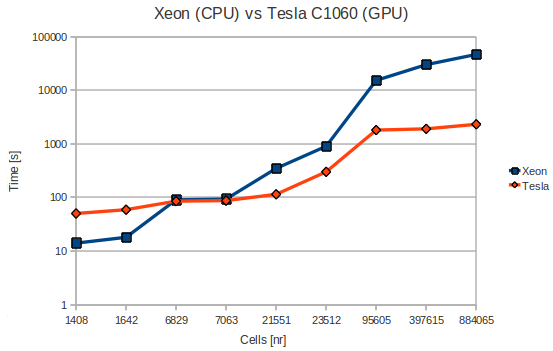
\includegraphics[width=0.7\textwidth]{img/XeonVsTesla.png}}
	\caption{Performance comparison between Intel Xeon and Nvidia Tesla.}
	\label{fig:NvidiaGPUsLogicalOrg}
\end{figure}

\section{Benchmark 2: GPU Occupancy}

\section{Benchmark 3: GPU Throughput}


